\chapter{Soluciones coloidales}

%%%%%%%%%%%%%%%%%%%%%%%%%%%%%%%%%%%%%%%%%%%%%%%%%%
\section{Introducci\'on}

En los \'ultimos cap\'itulos, hemos hecho hincapi\'e en la importancia y el potencial uso de los geles polim\'ericos. Dado el tema de investigaci\'on de esta tesis nos hemos enfocado especialmente en su aplicaci\'on para el secuestro de prote\'inas y/o f\'armacos de inter\'es terap\'eutico.
En este sentido, en los dos \'ultimos cap\'itulos hemos presentado dos tipos de modelos que permiten estudiar la fisicoqu\'imica de un nano/microgel aislado en soluci\'on.
En el cap\'itulo  \ref{Chapter-geles} hemos hecho referencia a un modelo robusto, un modelo de dos fases, con el cual logramos explicar la respuesta de los microgeles con respuesta a  m\'ultiples est\'imulos. Como los cambios en pH, temperatura o concetraci\'on de sal afectan a la capacidad de adsorber y liberar distintas moleculas, as\'i como sus cambios de tama\~no y carga. 
En el siguiente cap\'itulo,\ref{Chapter-esfericas} , se ha complejizado nuestro modelo para investigar c\'omo la estructura interna afecta la respuesta de estos geles. Al hacer esto obtuvimos nueva informaci\'on que no era accesible con el modelo anterior: localizaci\'on de la adsorci\'on y reordenamiendo de la estructura interna de los geles debido a est\'imulos externos.
Con el modelado propuesto en cap\'itulo \ref{Chapter-esfericas}  se ha podido  demostrar  que el dise\~no de la estructura de los nanogeles,  pensar en distintas estrateg\'ias de  s\'intesis, son factores importantes para optimizar los procesos de encapsulaci\'on y liberaci\'on de prote\'inas. 
Siendo este uno de los primeros pasos, a nivel experimental, para el dise\~no de trasnportadores de drogas.

Para poder acercanos m\'as a estos modelos experimentales damos un paso hacia las soluciones de nanogeles. En los cap\'itulos previos se han consideras geles aislados, o en un dilusi\'on infinita.
En este \'ultimo cap\'itulo,  indagaremos la fisicoqu\'imica de las soluciones de nanogeles. Como se ven afectados los comportamientos individuales, ya reportados en los cap\'itulos anteriores, ahora en funci\'on de la cantidad de ellos en soluci\'on, es decir que tan concentrados se encuentren la soluci\'on.
En esta primera aproximaci\'on usamos como m\'etodo de estudio simulaciones del tipo MonteCarlo y como referencia se utiliza el modelo y teor\'ia del sistema de dos fases presentado en el cap\'itulo \ref{Chapter-geles}. En la siguiente secci\'on mostraremos c\'omo lo incorporamos y hablamos de ``modelo de referencia''. 

\section{M\'etodo: Simulaci\'on Monte Carlo}


La simulaci\'on de sistemas de nanogeles en soluci\'on es una herramienta invaluable para comprender su comportamiento y sus propiedades termodin\'amicas. En este estudio, se emple\'o el m\'etodo Monte Carlo, en particular el algoritmo de Metropolis-Monte Carlo, para modelar la soluci\'on de nanogeles.
El m\'etodo de Metropolis-Monte Carlo \addcite se fundamenta en la generaci\'on aleatoria de n\'umeros y la evaluaci\'on de distintos estados o configuraciones del sistema en estudio. En cada paso de la simulaci\'on, se selecciona de manera aleatoria una configuraci\'on y se calcula su energ\'ia o probabilidad seg\'un un modelo predefinido. Este modelo debe poder describir las interacciones entre los componente del sistema, en nuestro caso son las part\'iculas de nanogeles y el solvente.
La simulaci\'on Monte Carlo, mediante el algoritmo de Metropolis-Monte Carlo nos ofrece una perspectiva \'unica para explorar las propiedades de los nanogeles en soluci\'on y su comportamiento en diferentes condiciones. 
En el caso espec\'ifico de nuestra soluci\'on de nanogeles, una configuraci\'on consiste en el movimiento y aumento de tama\~no de una part\'icula (nanogel) seleccionada al azar. 
\textcolor{red}{agregar esquema de paso de simulaci\'on.}

\includegraphics[width=10cm]{example-image-a} 

En este sentido la probabilidad de acetar o no dichos cambios en el sistema biene dado por:

\begin{align}
	P(s) = min \{e^{-(\Delta U^s_{inter} + \Delta U^s_{intra})},1\}
\end{align}

En donde $P(s)$ indica la probabilidad de aceptaci\'on del estado $s$, este estado consta de un cambio en el tama\~no y posici\'on de una nanogel. $\Delta U^s_{intra}$ corresponde al cambio en la energ\'ia interna de cada nanogel, debido a un cambio en su tama\~no, la energ\'ia de estos estados es obtenida usando una teor\'ia termodin\'amica detallada en el cap\'itulo  \ref{Chapter-geles}. El modelo de dos fases nos permite obtener la informaci\'on termodin\'amica necesarioa para explicar el comportamiento de una nanogel aislado.
El costo energetico de adsorber solvente, con sus respectivo iones, energ\'ia el\'astica, entrop\'ias de mezcla, entre otros (discutidos en el cap. \ref{Chapter-geles}).
En particular la energ\'ia que se toma de referencia correspoden a las de la figura \ref{fig:gel:graph-min} que nos muestra como cambia la energ\'ia del microgel(para esta figura) en funci\'on de su tama\~no.
Los resultados que mostraremos m\'as adelante correponden a nanogeles, tama\~no menor a 200 nm.
La energ\'ia interna de estos geles puede verse en la . La cual correspone a un nanogel con $2\times10^5$ mon\'omeros totales reparticos en 200 cadenas. \textcolor{red}{figura de $\Omega/V$ vs R}

\begin{figure*}[!tb]
	\centering
	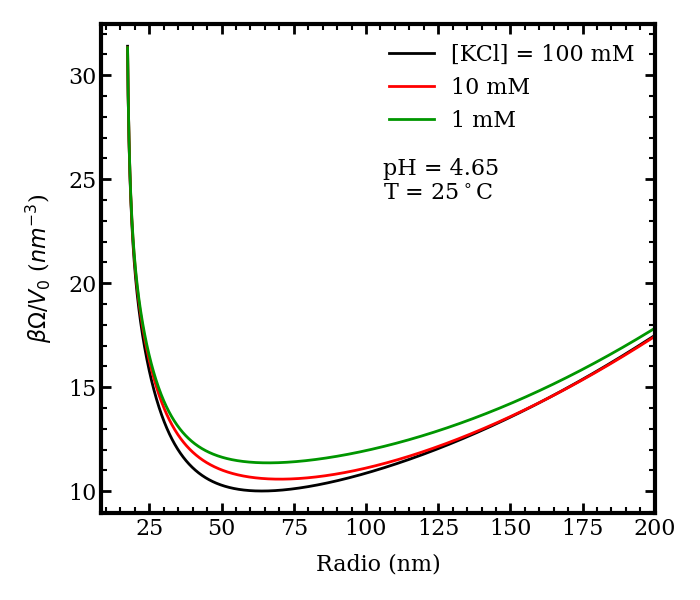
\includegraphics[width=1\linewidth]{Figures/graph-mc/interna.png}
	\caption{Energ\'ia interna para los cambios de tamaño de un nanogel...}
	\label{fig:mc:omega}
\end{figure*}


Por otro lado la energ\'ia intermolecular, $\Delta U_{inter}$, viene dada por la interacci\'ion de a pares de todos los nanogeles en soluci\'on. 
Para esta interacci\'on de a pares se ha utilizado un potencial combinado: Hertz-Yukawa. Este potencial fue previamente utilzado en \addcite[weyer2018concentration], en los cuales \addcite[weyer2018concentration] 
estudiaron la hinchaz\'on y las propiedades estructurales de suspensiones de microgeles i\'onicos su teor\'ia inlcuye las interacciones el\'asticas efectivas de Hertz y una teor\'ia de interacciones electrost\'aticas efectivas dependientes de la densidad (Yukawa). 
(un poco m\'as de los potenciales)
\textcolor{red}{Porque los podemos usar para nuestro sistema..}
Estamos trabajamos con materiales blandos que son deformables, por tando es posible modelarlos usando un potencial de Hertz, en el cual se considera la superposici\'on de las part\'iculas involucradas.
Yukawa por su parte es un potencial del tipo columbico mediado por el medio dilectrico en el que se encuentra. Se ven involucradas las cargas que envuelven a cada nanogel considerando la longitud de Debye. 
Podemos resumir nuestro potencial total de trabajo como:

\begin{align}
	U_{inter}(r) = \begin{cases} U_H + U_Y & \text{if } r \leq a_i + a_j \\ U_Y & \text{if } r > a_i + a_j \end{cases} 
	\label{eq:HY-potential}
\end{align}

en donde $r$ es la distancia entre dos nanogeles, definida como la distancia de sus centros. 
$a_i$ y $a_j$ representan los radios de el nanogel $i$ y $j$ respectivamente. Por ello la condici\'on $r \leq a_i +a_j$ representa la superposici\'on de estas particulas, deformandose y entrando en juego el potencial de Hertz.
Para mayores distancia a la suma de los radios de cada nanogel se pone en juego el potencial de Yukawa. Para el cual se define:
\begin{align}
	\beta u_Y(r) = q_i q_j \frac{e^{\kappa(a_i + a_j)}}{(1 +\kappa a_i)(1 + \kappa a_j)} \frac{e^{-\kappa r}}{r} 
	\label{eq:yukawa}
\end{align}

En donde $q_i$ y $q_j$ son las cargas netas que poseen los nanogeles $i$ y $j$ respectivamente. El valor $\kappa$ corresponde a la constante de apantallamiento de Debye. 
El pontecial de Hertz, $U_H$, se define como:
 

\begin{align}
	\begin{aligned}
		& \beta u_H (r) = \left(\frac{1-r}{a_i + a_j}\right)^{5/2}\times b_{12} \\
	\end{aligned}
\end{align}


En donde $b_{12}$ es la constante de interacci\'on entre las part\'iculas la cual depende de las propiedades el\'asticas del nanogel a trav\'es del m\'odulo de Young $\Lambda$ y el radio de Poisson $\nu$. \addcite[landau] La teor\'ia de escalado en sistemas de redes polim\'ericas predice que en buenos solventes \addcite que el m\'odulo de Young  escala linealmente con la temperatura y la densidad de los entrecruzamientos (o n\'umero de cadenas): $\Lambda \approx TN_{ch}/v$. Cuanto m\'as densos sean los entrecruzamientos, m\'as r\'igido ser\'a el gel.
Con lo cual podemos definir $b_{12}^\ast = \beta b_{12}$ el cual nos independiza de la temperatura y solo tenemos la dependencia con el n\'umero de cadenas ($N_{ch}$) y grado de entrecruzamiento de nuestro nanogel. 


\subsection{Potencial zeta ($\zeta$)}


Adem\'as de poder observar las fluctuasiones en los cambio de tamaño de los nanogeles es posible el calculo de ciertas propiedades de las mismas. Entre ellas estan el potencial zeta ($\zeta$).
Este potencial se define como...
El potencial zeta es una medida de la carga el\'ectrica neta en la superficie de una part\'icula coloidal, en este caso un nanogel. El potencial zeta afecta la estabilidad de las part\'iculas coloidales, su viscosidad y su interacci\'on con otras part\'iculas.
En los nanogeles, el potencial zeta se genera por las cargas el\'ectricas de las cadenas polim\'ericas que forman la red del gel. Las cadenas  pueden tener carga positiva o negativa, dependiendo de los grupos funcionales que contengan. De este modo el potencial zeta puede ser positivo, negativo o neutro.

El potencial zeta de un nanogel afecta su estabilidad de varias maneras. Cuando el potencial zeta es positivo, los nanogel se repelen entre s\'i, lo que hace m\'as estable en soluci\'o. Cuando el potencial zeta es negativo, las part\'iculas del nanogel se atraen entre s\'i, lo que puede hacer que los nanogeles se aglomeren.
Las cargas negativas de las superficies de los nanogeles no est\'an directamente en contacto entre s\'i. Estas cargan se ecuentran  separadas por una capa de agua. El agua tiene una carga positiva neta, por lo que las cargas negativas de los nanogeles son atra\'idas por la capa de agua. Esta atracci\'on es m\'as fuerte que la repulsi\'on entre las cargas negativas, por lo que los nanogeles se aglomeran.

Luego el potencial zeta puede definirse como: \addcite[libro S\&C]

\begin{align}
	\zeta (a) \propto \frac{Z_{net}}{a} \frac{1}{1 +ka}
	\label{eq:mc:potzeta}
\end{align}


\noindent en donde  $k$ es la inversa de la lingitud de Debye, $a$ es el radio del nanogel y $Z_{net}$ es la carga neta que se observa del nanogel al considerarlo como un nano-ion \addcite[Denton 2003]. Esta carga se deriva de la interacci\'on electrost\'atica que ocurre con la part\'icula y los contraiones que lo rodean:
\begin{align}
	Z_{net}(a) = (1 + ka)e^{-ka} \frac{3Z}{k^2a^2}\left(\cosh(ka) - \frac{\sinh(ka)}{ka}\right)
	\label{eq:mc:znet}
\end{align}

\noindent en donde $Z$ es definida como la carga orginada por el grado de carga de los segmentos cargados que componen al nanogel.

\section{Fluctuaci\'on en Volumen} \label{sec:mc:fluctuacion}
Se define la fluctuaci\'on en volumen como:
\begin{align}
	\frac{\Delta V}{V} = \sqrt{\frac{k_BT}{V}\kappa_T}
\end{align}

\noindent en donde $\kappa_T$ es la incompresiblidad isot\'ermica, la cual se obtiene:

\begin{align}
	\begin{aligned}
		\kappa & = -\frac{1}{V} \left( \frac{\partial V}{\partial P}\right)_T \\
		& =\frac{1}{V} \left( \frac{\partial^2 \Omega}{\partial V^2}\right)^{-1}_T \\
		& = 12 \pi R_{eq} \left( \frac{\partial^2 \Omega}{\partial R^2}\right)^{-1}_{T,R=R_{eq}}
	\end{aligned}
\end{align}


\section{Resultados}


\begin{figure*}[!tb]
	\centering
	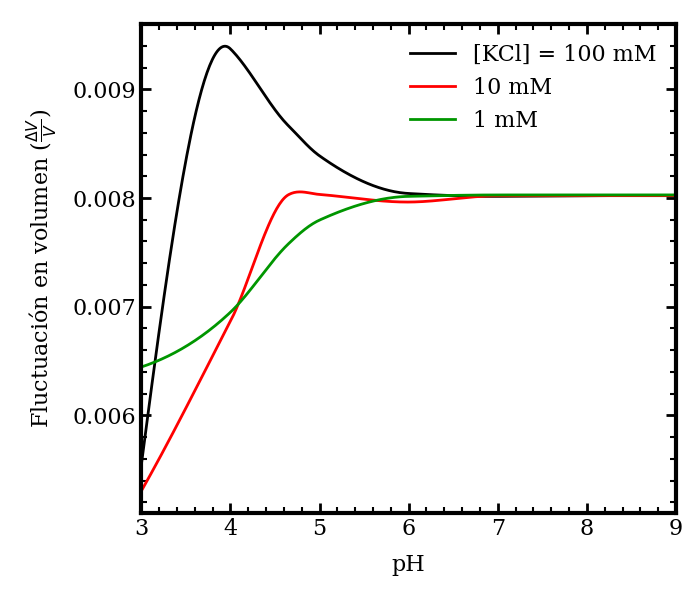
\includegraphics[width=1\linewidth]{Figures/graph-mc/dvv.png}
	\caption{Gr\'afico de la fluctuaci\'on en volumen de un nanogel aislado. El nanogel esta compuesto por $2\times 10^5$ segmentos (mon\'omeros) repartidos en 200 cadenas de 1000 cadenas cada una.}
	\label{fig:mc:dvvi}
\end{figure*}
En la figura \ref{fig:mc:dvvi} se observa la fluctuaci\'on en tama\~no de un nanogel aislado, la energ\'ia libre de estos sistemas es calcula usando el modelo del cap\'itulo \ref{Chapter-geles}....
La temperatura es de $25 ^\circ C$ condiciones en las cuales el NIPAM es hidrofilico y por ello las fluctuaciones mostradas en esta figura no se ven afectadas por la presencia de este co-mon\'omero.

C\'omo se puede observar la fluctuaci\'on del sistema diferentes condiciones de pH y concentraci\'on salina son despreciables. el c\'alculo de las mismas se realizaron con  lo expresado en la secci\'on \ref{sec:mc:fluctuacion}.
Dentro de estos valores de fluctuaci\'on se puede observar un aumento de la misma al aumentar el pH hasta estabilizar en valores de pH alrededor de 6.
A bajos valores de pH el nanogel no posee carga, los mon\'omeros de MAA que los componen se ecuentran desprotonados (estamos por debajo del pKa intr\'inseco del MAA) en estas condiciones un cambio en el tama\~no del nanogel con lleva la absorci\'on o liberaci\'on de solvente y de los iones presentes en el, adem\'as de la energ\'ia el\'astica que conlleva el cambio de radio.
La entrada o salida de iones conlleva un cambio en la cantidad de carga dentro del nanogel con lo cual se esperar\'ia un aumento en el grado de carga de los mon\'omeros, en estas condiciones de pH es muy desfavorable la desprotonaci\'on de la red polim\'erica. En consecuencia las fluctuaciones son las m\'as bajas de todo el rango de pHs.
En part\'icular altas concentraciones salinas promueven una desprotonaci\'on de los segmentos de MAA para peque\~nos aumentos de pH, ver figura \ref{fig:gel:f-cs}B, con lo cual la entrada de iones favorece la fluctuaci\'on en volumen del nanogel. 
Por otro lado a condiciones de pH altos, el gel se encuentra con un alto grado de carga. La salida o entrada de iones, y  con lo cual podr\'ia surgir un cambio en la carga del nanogel,  es m\'as favorable que a bajos pH y por ello se observa una fluctuaci\'on mayor. En estos valores altos de pH no hay diferencia alguna con la concentraci\'on salina. El nanogel posee tanta carga que los cambios en la salinidad no afectan a las flutuaciones.





\begin{figure*}[!tb]
	\centering
	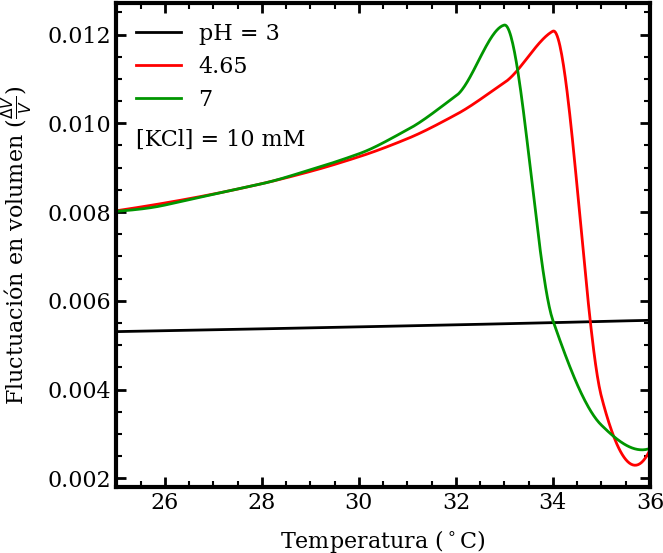
\includegraphics[width=1\linewidth]{Figures/graph-mc/fluct-T.png}
	\caption{Gr\'afico de la fluctuaci\'on en volumen de un nanogel aislado. El nanogel esta compuesto por $2\times 10^5$ segmentos (mon\'omeros) repartidos en 200 cadenas de 1000 cadenas cada una.}
	\label{fig:mc:dvv-Ti}
\end{figure*}

En la figura \ref{fig:mc:dvv-Ti} mostramos la fluctuaci\'on en volumen originada al cambiar la temperatura del sistema. Para esta figura revisaremos como se ven afectados los cambios en el tama\~no del nanogel debido al colapso de la red polim\'erica por la hidrofibicidad surgida al aumentar la temperatura. Adem\'as se presentan tres curvas mostrando los tres pH caracter\'isticos del sistema. Por abajo y arriba del pH intr\'insico pH 3 y 7 respectivamente y uno al valor del pKa del MAA aislado.
Para el pH 3 el grado de carga del gel es pr\'acticamente nulo, ver figura \ref{fig:gel:f-cs}B, por lo cual las fluctuaciones que se observan son por efecto de la temperatura. Al aumentar la temperatura se le agrega energ\'ia al sistema. Observ\'andose as\'i una peque\~na pendiente en dicha curva.

A pH 4.65 y 7 el sistema posee carga por tanto al agregarle energ\'ia al sistema (aumento de temperatura) las fluctuaciones aumentan. Esto ocurre hasta llegar a la temperatura caracter\'istica de transici\'on volum\'etrica del NIPAm, figura \ref{fig:gel:R-T}, por arriba de los $32 ^\circ$C. Despu\'es de este punto hay un colapso en la estructura del nanogel con lo cual es poco probable que se de un cambio de su tama\~no en un punto en part\'icular. ase observa un decaimiento de las fluctuaciones. 

\begin{figure*}[!tb]
	\centering
	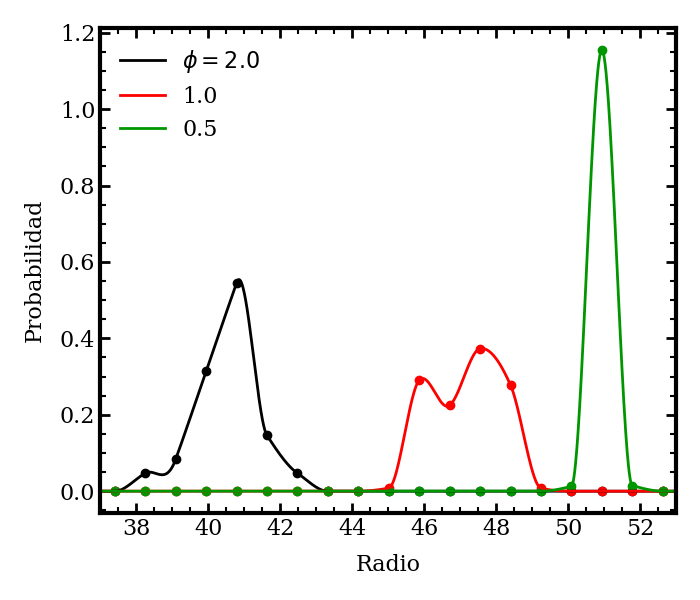
\includegraphics[width=1\linewidth]{Figures/graph-mc/denton.png}
	\caption{Gr\'afico del probabilidad de tama\~no de la soluci\'on de  nanogeles en funci\'on de la densidad... fracci\'on de volumen ocupada. nanogel m\'as flexible... 200 monomeros por cadena. 2e5 monomeros totales. radio medio aisladop = 51 nm }
	\label{fig:mc:dentos-sizes}
\end{figure*}
